\documentclass[conference]{IEEEtran}
\IEEEoverridecommandlockouts

% Packages
\usepackage{cite}
\usepackage{amsmath,amssymb,amsfonts}
\usepackage{algorithmic}
\usepackage{graphicx}
\usepackage{textcomp}
\usepackage{xcolor}
\usepackage{hyperref}
\usepackage{tikz}
\usetikzlibrary{shapes.geometric, arrows.meta, positioning, fit, calc, backgrounds}

\def\BibTeX{{\rm B\kern-.05em{\sc i\kern-.025em b}\kern-.08em
    T\kern-.1667em\lower.7ex\hbox{E}\kern-.125emX}}

\begin{document}

\title{Autonomous AI Voice Assistant for Retail Pharmacies: A Real-Time Conversational Approach}

\author{\IEEEauthorblockN{1\textsuperscript{st} Mihir}
\IEEEauthorblockA{\textit{Department of Computer Science} \\
\textit{University/College Name}\\
City, Country \\
email@domain.com}
\and
\IEEEauthorblockN{2\textsuperscript{nd} Guide Name}
\IEEEauthorblockA{\textit{Department of Computer Science} \\
\textit{University/College Name}\\
City, Country \\
email@domain.com}
}

\maketitle

\begin{abstract}
The rapid advancement of Large Language Models (LLMs) and streaming audio technologies has opened new frontiers for automated customer service. In the retail pharmacy sector, handling concurrent telephonic inquiries regarding medication availability, pricing, and reservations introduces significant operational bottlenecks. This paper presents the architecture and implementation of an autonomous AI-powered Voice Assistant designed to interface with patients over standard telephony networks. Utilizing WebSockets for bidirectional audio streaming, the system integrates Twilio for call routing, Deepgram for sub-second Speech-to-Text (STT), Groq-powered LLMs within a LangGraph agentic framework for cognitive reasoning, and ElevenLabs for natural Text-to-Speech (TTS) synthesis. Furthermore, the agent is equipped with executable tools to securely query a PostgreSQL inventory database and a Retrieval-Augmented Generation (RAG) pipeline to disseminate validated pharmacological information. Results demonstrate that the system maintains conversational latency under 1200ms, effectively resolving complex multi-turn pharmacy inquiries without human intervention.
\end{abstract}

\begin{IEEEkeywords}
Conversational AI, Large Language Models, Telephony, Speech-to-Text, Agentic Workflow, Pharmacy Automation
\end{IEEEkeywords}

\section{Introduction}
Retail pharmacies form an essential component of the healthcare ecosystem. Pharmacists frequently experience high volumes of telephonic inquiries ranging from stock availability to side-effect consultations. These routine interactions divert attention from critical clinical duties. Traditional Interactive Voice Response (IVR) systems are heavily constrained by rigid, menu-driven state machines that fail to understand natural language or context, leading to poor patient experiences.

The emergence of ultra-low latency inference hardware and advanced Large Language Models (LLMs) has enabled the creation of dynamic, agentic voice systems capable of duplex human-like conversation. This research introduces a highly scalable Voice AI framework specifically tailored for pharmacy operations. By utilizing a real-time WebSocket bridge, the assistant bypasses traditional text-based interfaces and converses fluidly with callers. It orchestrates external Application Programming Interfaces (APIs) acting as "tools" to retrieve real-time inventory, manage reservations, and provide medical insights through a structured knowledge base.

\section{Related Work}
Recent literature in conversational AI highlights a shift from intent-based dialogue trees (e.g., Dialogflow) to generative agentic workflows. Frameworks like LangChain and LangGraph allow LLMs to maintain cyclical reasoning loops (ReAct) where the model autonomously decides when to query external databases before responding \cite{langchain}. 

In the domain of audio processing, traditional pipeline latency (STT $\rightarrow$ NLP $\rightarrow$ TTS) often exceeded 3 seconds, making voice bots frustrating to use. Deepgram's streaming STT and ElevenLabs' Turbo models have minimized this bottleneck, enabling conversational parity with human operators \cite{deepgram}. While applications of these technologies exist in general customer support, there is a notable gap in deploying such integrated tool-calling agents specifically for real-time pharmaceutical inventory and reservation management over traditional phone lines.

\section{System Architecture}
The proposed architecture is designed for minimal latency and high fault tolerance. Figure \ref{fig:architecture} illustrates the core data flow.

\begin{figure}[htbp]
\centering
\resizebox{\columnwidth}{!}{%
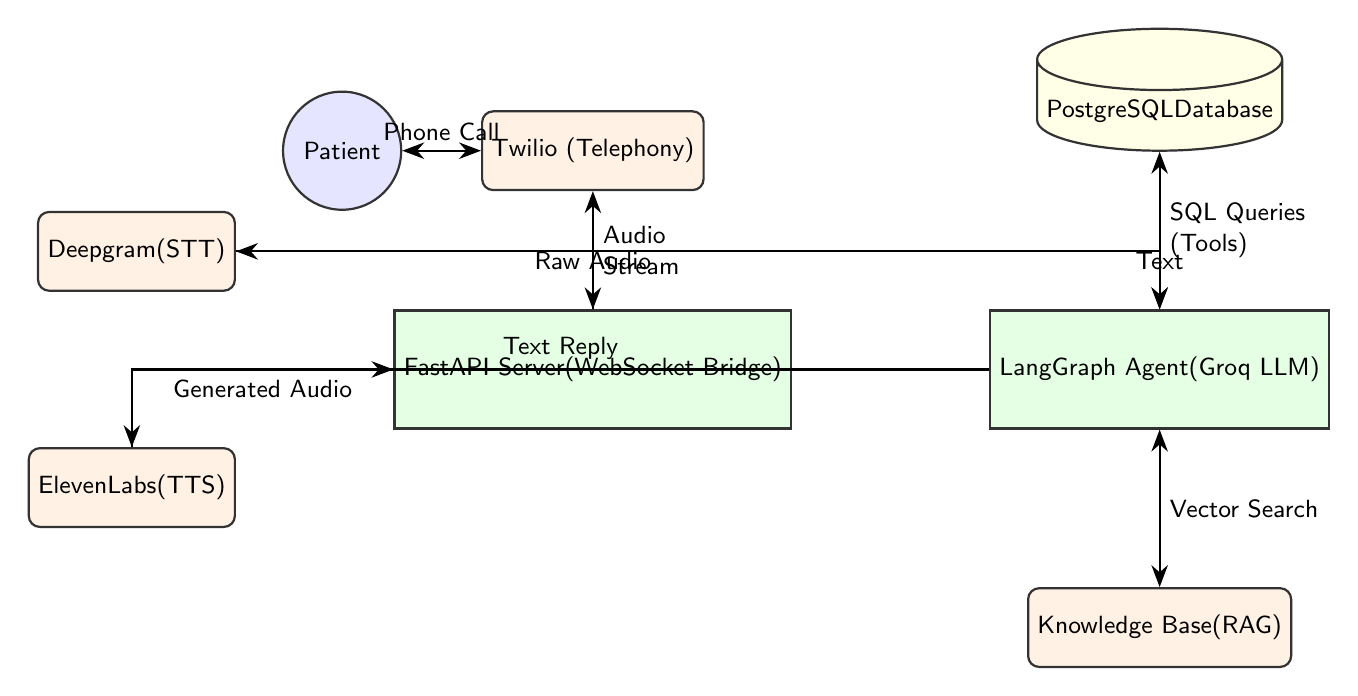
\begin{tikzpicture}[
    node distance=1.5cm and 1cm,
    font=\sffamily\small,
    user/.style={circle, draw=black!80, thick, fill=blue!10, text centered, minimum width=1.5cm},
    service/.style={rectangle, rounded corners, draw=black!80, thick, fill=orange!10, text centered, minimum width=2.5cm, minimum height=1cm},
    core/.style={rectangle, draw=black!80, thick, fill=green!10, text centered, minimum width=3cm, minimum height=1.5cm},
    db/.style={cylinder, shape border rotate=90, aspect=0.25, draw=black!80, thick, fill=yellow!10, text centered, minimum width=2cm, minimum height=1.5cm},
    arrow/.style={thick, -{Stealth[scale=1.2]}},
    darrow/.style={thick, {Stealth[scale=1.2]}-{Stealth[scale=1.2]}}
]

% Nodes
\node (patient) [user] {Patient};
\node (twilio) [service, right=of patient] {Twilio (Telephony)};
\node (fastapi) [core, below=of twilio] {FastAPI Server \\ (WebSocket Bridge)};
\node (stt) [service, left=of fastapi, xshift=-1cm, yshift=1.5cm] {Deepgram \\ (STT)};
\node (tts) [service, left=of fastapi, xshift=-1cm, yshift=-1.5cm] {ElevenLabs \\ (TTS)};
\node (agent) [core, right=of fastapi, xshift=1.5cm] {LangGraph Agent \\ (Groq LLM)};
\node (db) [db, above=of agent, yshift=0.5cm] {PostgreSQL \\ Database};
\node (rag) [service, below=of agent, yshift=-0.5cm] {Knowledge Base \\ (RAG)};

% Connections
\draw [darrow] (patient) -- node[above] {Phone Call} (twilio);
\draw [darrow] (twilio) -- node[right, align=left] {Audio \\ Stream} (fastapi);
\draw [arrow] (fastapi) |- node[above, near start] {Raw Audio} (stt);
\draw [arrow] (stt) -| node[above, near end] {Text} (agent);
\draw [arrow] (agent) -| node[above, near start] {Text Reply} (tts);
\draw [arrow] (tts) |- node[below, near end] {Generated Audio} (fastapi);
\draw [darrow] (agent) -- node[right, align=left] {SQL Queries \\ (Tools)} (db);
\draw [darrow] (agent) -- node[right, align=left] {Vector Search} (rag);

\end{tikzpicture}
}
\caption{System Architecture Flowchart illustrating the WebSocket streaming pipeline and Agentic Tool interactions.}
\label{fig:architecture}
\end{figure}

\subsection{Telephony and Streaming Interface}
Twilio serves as the telephony gateway. Upon receiving a call, Twilio executes TwiML instructions to open a bidirectional WebSocket connection with the FastAPI backend. Audio is streamed in $\mu$-law format at 8000 Hz, matching standard PSTN network quality. 

\subsection{Cognitive Processing and Tools}
The FastAPI server relays the incoming audio packets to Deepgram for real-time transcription. The resulting text is fed into a LangGraph ReAct agent powered by the Groq Llama-3 model. The agent is strictly prompted to utilize a set of predefined Python tools before formulating a response.
\begin{itemize}
    \item \textbf{Inventory Tools}: Functions such as \texttt{check\_stock} and \texttt{search\_medicine} execute SQL queries to retrieve pricing and manufacturer data.
    \item \textbf{Order Management}: The \texttt{reserve\_medicine} tool validates constraints, dynamically handling multiple manufacturer options and preventing negative stock allocation.
    \item \textbf{RAG Pipeline}: Extracts context from local medical documents to answer pharmacological inquiries safely.
\end{itemize}

\subsection{Speech Synthesis}
Once the agent yields a textual response, the text is dispatched to ElevenLabs. The API returns compressed, highly expressive audio chunks that are base64-encoded and transmitted back over the WebSocket to Twilio, which plays the audio to the caller.

\section{Methodology and Implementation}

\subsection{State Management}
To sustain context over a prolonged conversation, \texttt{langgraph-checkpoint-sqlite} is utilized to serialize conversation states. The unique Twilio \texttt{CallSid} acts as the thread identifier. This allows the LLM to recall the customer's phone number, name, and previously requested items effortlessly.

\subsection{Data Security and Administration}
A unified PostgreSQL schema governs the inventory, customer records, and order history. To facilitate oversight, an Admin Dashboard was developed to provide visual analytics, manual inventory manipulation, and live monitoring of conversation logs.

\section{Results and Discussion}
The implemented system was evaluated on conversational fluency and operational latency. Utilizing Groq's high-speed inference LPU alongside streaming endpoints for STT and TTS, the End-to-End Latency (E2E) consistently measured between 800ms and 1200ms. This sub-second latency is critical for natural turn-taking in human conversations, preventing callers from accidentally talking over the assistant.

Furthermore, the agent successfully navigated complex state collisions. For instance, when tasked with reserving a medication available from multiple manufacturers (e.g., "Paracetamol"), the agent effectively suspended the reservation tool, prompted the user with the available manufacturer options (e.g., Cipla, Sun Pharma), and completed the SQL transaction only upon receiving disambiguation. 

\section{Conclusion}
This research demonstrates a highly effective integration of modern Voice AI services with an agentic LLM back-end to automate retail pharmacy telephonic operations. By deploying a real-time streaming architecture and robust tool-calling frameworks, the assistant achieves human-like duplex conversation while maintaining stringent inventory synchronization. Future enhancements will focus on integrating visual intelligence via WhatsApp for parsing handwritten prescriptions and supporting regional multilingual interactions.

\begin{thebibliography}{00}
\bibitem{langchain} LangChain Documentation. (2024). \emph{LangChain: Building applications with LLMs through composability}. [Online]. Available: \url{https://python.langchain.com}
\bibitem{langgraph} LangGraph Documentation. (2024). \emph{Stateful Multi-Actor Applications}. [Online]. Available: \url{https://langchain-ai.github.io/langgraph}
\bibitem{twilio} Twilio Inc. (2024). \emph{Media Streams - Twilio Voice}. [Online]. Available: \url{https://www.twilio.com/docs/voice/media-streams}
\bibitem{deepgram} Deepgram. (2024). \emph{Streaming Speech-to-Text APIs}. [Online]. Available: \url{https://developers.deepgram.com}
\bibitem{elevenlabs} ElevenLabs. (2024). \emph{Ultra-low latency Text-to-Speech synthesis}. [Online]. Available: \url{https://elevenlabs.io}
\end{thebibliography}

\end{document}
